\documentclass[border=10pt]{standalone}
\usepackage{pgfplots}
\pgfplotsset{compat=1.18}
\begin{document}
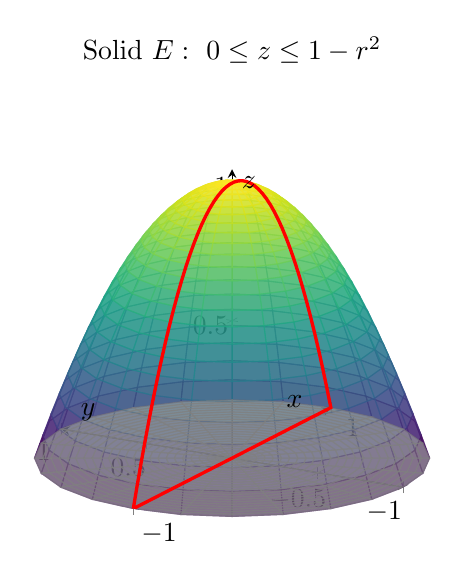
\begin{tikzpicture}
\begin{axis}[
    view={-60}{22},
    axis lines = middle,
    xlabel={$x$}, ylabel={$y$}, zlabel={$z$},
    domain=0:360, y domain=0:1,
    zmin=0, zmax=1.05,
    colormap/viridis,
    title={Solid $E:\ 0 \le z \le 1-r^2$},
]
% paraboloid surface z = 1 - r^2
\addplot3[surf, shader=flat, opacity=0.65, z buffer=sort]
    ({cos(x)*y}, {sin(x)*y}, {1-y^2});
% base disk z = 0
\addplot3[surf, shader=flat, color=gray, opacity=0.55, z buffer=sort]
    ({cos(x)*y}, {sin(x)*y}, {0});
% cross-section curve y = 0: z = 1 - x^2
\addplot3[very thick, color=red, domain=-1:1, samples=50]
    ({x}, 0, {1-x^2});
\end{axis}
\end{tikzpicture}
\end{document}